\documentclass[12pt]{article}
\usepackage[utf8]{inputenc}
\usepackage[spanish]{babel}
\decimalpoint
\usepackage{amsmath}
\usepackage{caption}
\usepackage{amsthm}
\usepackage{amssymb}
\usepackage{graphicx}
\usepackage[margin=0.9in]{geometry}
\usepackage{fancyhdr}
\usepackage[inline]{enumitem}
\usepackage{float}
\usepackage{cancel}
\usepackage{bigints}
\usepackage{color}
\usepackage{xcolor}
\usepackage{listingsutf8}
\usepackage{algorithm}
\usepackage{tocloft}
\usepackage[none]{hyphenat}
\usepackage{graphicx}
\usepackage{grffile}
\usepackage{tabularx}
\usepackage[nottoc,notlot,notlof]{tocbibind}
\usepackage{times}
\usepackage{color}
\definecolor{gray97}{gray}{.97}
\definecolor{gray75}{gray}{.75}
\definecolor{gray45}{gray}{.45}
\renewcommand{\cftsecleader}{\cftdotfill{\cftdotsep}}
\pagestyle{fancy}
\setlength{\headheight}{15pt} 
\lhead{PRACTICA 1}
\rhead{\thepage}
\lfoot{ESCOM-IPN}
\renewcommand{\footrulewidth}{0.5pt}
\setlength{\parskip}{0.5em}
\newcommand{\ve}[1]{\overrightarrow{#1}}
\newcommand{\abs}[1]{\left\lvert #1 \right\lvert}
\date{26 de febrero de 2017}
\title{Pruebas a posteriori}
\author{Reporte 1}

\definecolor{pblue}{rgb}{0.13,0.13,1}
\definecolor{pgreen}{rgb}{0,0.5,0}
\definecolor{pred}{rgb}{0.9,0,0}
\definecolor{pgrey}{rgb}{0.46,0.45,0.48}
\lstset{tabsize=1}

\usepackage{listings}
\lstset{ frame=Ltb,
framerule=0pt,
aboveskip=0.5cm,
framextopmargin=3pt,
framexbottommargin=3pt,
framexleftmargin=0.4cm,
framesep=0pt,
rulesep=.4pt,
backgroundcolor=\color{gray97},
rulesepcolor=\color{black},
%
stringstyle=\ttfamily,
showstringspaces = false,
basicstyle=\small\ttfamily,
commentstyle=\color{gray45},
keywordstyle=\bfseries,
%
numbers=left,
numbersep=15pt,
numberstyle=\tiny,
numberfirstline = false,
breaklines=true,
}

% minimizar fragmentado de listados
\lstnewenvironment{listing}[1][]
{\lstset{#1}\pagebreak[0]}{\pagebreak[0]}

\lstdefinestyle{consola}
{basicstyle=\scriptsize\bf\ttfamily,
backgroundcolor=\color{gray75},
}

\lstdefinestyle{Java}
{language=Java,
}

%%%%%%%%%%%%%%%%%%%%%

\lstdefinestyle{customc}{
  belowcaptionskip=1\baselineskip,
  breaklines=true,
  frame=L,
  xleftmargin=\parindent,
  language=C,
  showstringspaces=false,
  basicstyle=\footnotesize\ttfamily,
  keywordstyle=\bfseries\color{green!40!black},
  commentstyle=\itshape\color{purple!40!black},
  identifierstyle=\color{blue},
  stringstyle=\color{orange},
}

\lstdefinestyle{customasm}{
  belowcaptionskip=1\baselineskip,
  frame=L,
  xleftmargin=\parindent,
  language=[x86masm]Assembler,
  basicstyle=\footnotesize\ttfamily,
  commentstyle=\itshape\color{purple!40!black},
}

\lstset{escapechar=@,style=customc}


    % =====  CODE EDITOR =========
    \lstdefinestyle{CompilandoStyle} {                              %This is Code Style
        backgroundcolor=\color{BlueGrey800MD},                      %Background Color  
        basicstyle=\tiny\color{white},                              %Font color
        commentstyle=\color{BlueGrey100MD},                         %Comment color
        stringstyle=\color{TealMD},                                 %String color
        keywordstyle=\color{Green100MD},                            %keywords color
        numberstyle=\tiny\color{TealMD},                            %Size of a number
        frame=shadowbox,                                            %Adds a frame around the code
        breakatwhitespace=true,                                     %Style                       
        breaklines=true,                                            %Style                   
        keepspaces=true,                                            %Style                   
        numbers=left,                                               %Style                   
        numbersep=10pt,                                             %Style 
        xleftmargin=\parindent,                                     %Style 
        tabsize=4                                                   %Style 
    }
 
    \lstset{style=CompilandoStyle}                                  %Use this style

    \usepackage{minted} % Paquete que permite citar codigo
    \usemintedstyle{borland} % Aqui se define el colorscheme para minted
    \setminted{
        fontsize = \scriptsize, % Ajusta el codigo a la hoja
        baselinestretch = 1,
        linenos, % set numbers
        breaklines=true, % Hace un salto de linea automatico en caso de que se llege al final de la line
        tabsize=3 
    }

%Permite crear columnas en el documento
\usepackage{multicol} 
\usepackage{color}
\usepackage{comment}
\newcommand{\tabitem}{~~\llap{\textbullet}~~}
\newcommand{\subtabitem}{~~~~\llap{\textbullet}~~}

\bibliographystyle{IEEEtran}
\begin{document}
		\begin{titlepage}
			\begin{center}
				
				% Upper part of the page. The '~' is needed because \\
				% only works if a paragraph has started.
				
				\noindent
				\begin{minipage}{0.5\textwidth}
					\begin{flushleft} \large
						\includegraphics[width=0.3\textwidth]{../ipn.png}
					\end{flushleft}
				\end{minipage}%
				\begin{minipage}{0.55\textwidth}
					\begin{flushright} \large
						\includegraphics[width=0.7\textwidth]{../escom.png}
					\end{flushright}
				\end{minipage}
				
				\textsc{\LARGE Instituto Politécnico Nacional}\\[0.5cm]
				
				\textsc{\Large Escuela Superior de Cómputo}\\[1cm]
				
				% Title
				
				{ \huge Práctica 1 - Pruebas a posteriori (Algoritmos de Ordenamiento)\\[1cm] }
				
				{ \Large Unidad de aprendizaje: Análisis de Algoritmos} \\[1cm]
				
				{ \Large Grupo: 3CM3} \\[1cm]
				
				\noindent
				\begin{minipage}{0.5\textwidth}
					\begin{flushleft} \large
						\emph{Alumnos(a): "La naranja mecánica"}\\
						
						\begin{tabular}{ll}
					     Nicolás Sayago Abigail\\
					     Parra Garcilazo Cinthya Dolores\\
					     Ramos Díaz Enrique \\
					
					\end{tabular}
					\end{flushleft}
				\end{minipage}%
				\begin{minipage}{0.5\textwidth}
					\begin{flushright} \large
						\emph{Profesor(a): Edgardo Adrián Franco Martínez} \\
						  \\
					\end{flushright}
				\end{minipage}
				
					\begin{minipage}{0.5\textwidth}
					\begin{center} \large
						\includegraphics[width=0.8\textwidth]{../xd.jpg}
						\caption*{"La Naranja Mecánica"}
					\end{center}
				\end{minipage}

				\vfill
				
				% Bottom of the page
				{\large 12 de Septiembre 2018}
			\end{center}
		\end{titlepage}
	
	\tableofcontents
	\newpage
	% /////////////////////////////////////////////////////////
	%			PLANTEAMIENTO DEL PROBLEMA
	% ////////////////////////////////////////////////////////
	\section{Planteamiento del problema}
	
    Existen diversos métodos de ordenamiento, en este documento se analizaran 5, se observara y comparará
    el comportamiento de cada uno, para determinar el mejor de todos.
    
    Este es el llamado Análisis a priori, en donde se tomaran resultados experimentales en una plataforma determinada para determinar la complejidad temporal y espacial de los siguientes algoritmos: Burbuja Simple, Burbuja Optimizada, Inserción, Selección, Shell y Árbol de Búsqueda Binario.
	
	% /////////////////////////////////////////////////////////
	%			PLATAFORMA EXPERIMENTAL
	% ////////////////////////////////////////////////////////
    \section{Plataforma Experimental}
    \textbf{Especificaciones de Hardware:}
    \begin{itemize}
        \item CPU: Intel Core-i5 6500 3.2 GHz
        \item Memoria: RAM DDR4 5.9 GB 2133 MHz
    \end{itemize}
    
    \textbf{Compilador:} GCC version 7.3.0 desde la Terminal
    
    \textbf{Sistema Operativo:} Linux Ubuntu 18.04.1 LTS x64 

	% /////////////////////////////////////////////////////////
	%			ACTIVIDADES Y PRUEBAS
	% ////////////////////////////////////////////////////////
	
	\section{Actividades y Pruebas}
	
		\subsection{Burbuja simple}
    		\subsubsection{Ejecución del algoritmo}
    		    \begin{figure}[H]
        	            \centering
        	             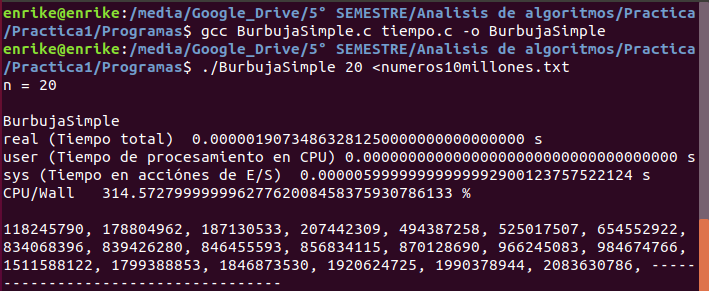
\includegraphics[scale=0.7]{images/Pruebas/burbujaSimple.png}
                \end{figure}
                
    		\subsubsection{Análisis Temporal}
    		    \begin{figure}[H]
        	            \centering
        	             \includegraphics[scale=0.9]{images/Tabla/BS.PNG}
                \end{figure}
                
    		\subsubsection{Gráfica de comportamiento}
    		    \begin{figure}[H]
        	            \centering
        	             \includegraphics[scale=0.8]{images/Graficas/BS.PNG}
                \end{figure}
            
    		\newpage
    		\subsubsection{Aproximaciones Polinomiales}
        		    \begin{figure}[h!]
                    \centering
                   \subfigure{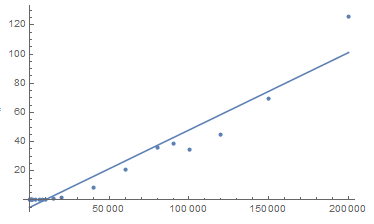
\includegraphics[width=0.61\textwidth]{Practica1/images/burbujapol1.PNG}
                   \caption*{\textbf{Grado 1: $-5.00391 + 0.000530695 x$}}}
    
    
                   \subfigure{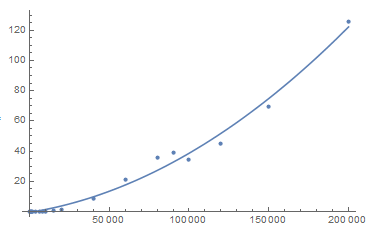
\includegraphics[width=0.61\textwidth]{Practica1/images/burbujapol2.PNG}
                   \caption*{\textbf{Grado 2: $-0.519656 + 0.0001691 x + 2.22402\times10^{-9} x^2$}}}
                   \\
        		  \subfigure{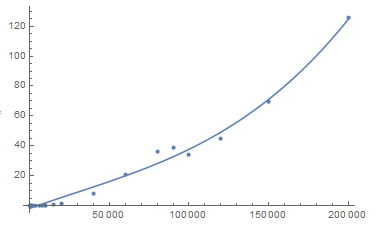
\includegraphics[width=0.61\textwidth]{Practica1/images/burbujapol3.PNG}
                   \caption*{\textbf{Grado 3: $-1.67871 + 0.000378947 x - 9.51029\times10^{-10} x^2 + 1.11022\times10^{-14} x^3$}}}
                   \end{figure}
                    \newpage
                   \begin{figure}[h!]
                    \centering
        		   \subfigure{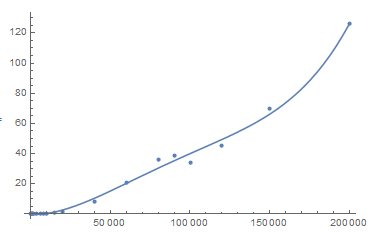
\includegraphics[width=0.61\textwidth]{Practica1/images/burbujapol4.PNG}
                   \caption*{\textbf{Grado 4: $-0.141273 - 0.0000406877 x + 1.08914\times10^{-8} x^2 - 9.16426\times10^{-14} x^3 + 2.70052\times10^{-19} x^4$}}}
                   
                   \subfigure{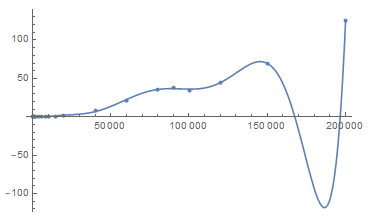
\includegraphics[width=0.61\textwidth]{Practica1/images/burbujapol8.PNG}
                   \caption*{\textbf{Grado 8:  $0.516742 - 0.000566326 x + 9.99756*10^-8 x^2 - 5.90874*10^-12 x^3 + 
                    1.70318\times10^{-16} x^4 - 2.50739\times10^{-21} x^5 + 1.94326\times10^{-26} x^6 - 
                     7.5416\times10^{-32} x^7 + 1.15235\times10^{-37} x^8$}}}
                \end{figure}
                \subsubsection{Evaluación de n's en Polinomios}
                \begin{figure}[H]
        	            \centering
        	             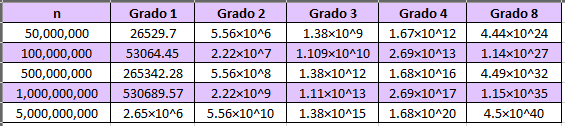
\includegraphics[scale=1]{images/NPols/nBS.PNG}
                \end{figure}
\newpage
            
		\subsection{Burbuja Optimizada}
    		\subsubsection{Ejecución del algoritmo}
        		\begin{figure}[H]
        	            \centering
        	            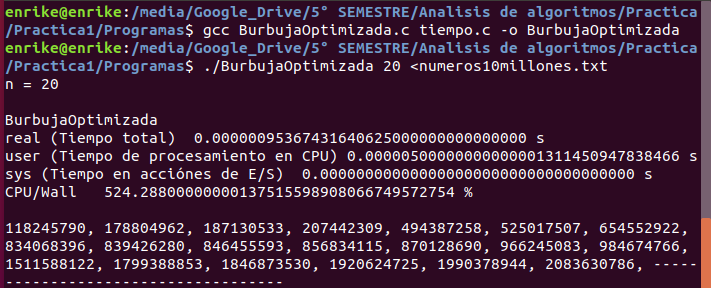
\includegraphics[scale=0.7]{images/Pruebas/bso.png}
                \end{figure}

    		\subsubsection{Análisis Temporal}
    		    \begin{figure}[H]
        	            \centering
        	             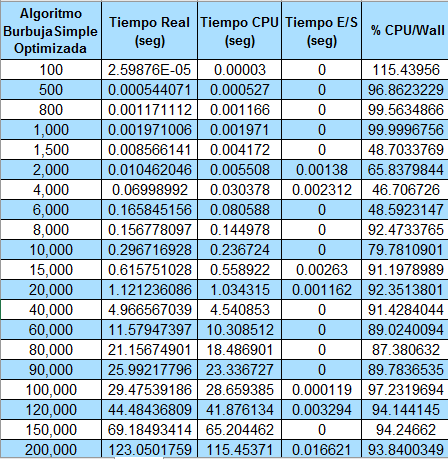
\includegraphics[scale=0.9]{images/Tabla/BSO.PNG}
                \end{figure}
    		\subsubsection{Gráfica de comportamiento}
    		    \begin{figure}[H]
        	            \centering
        	             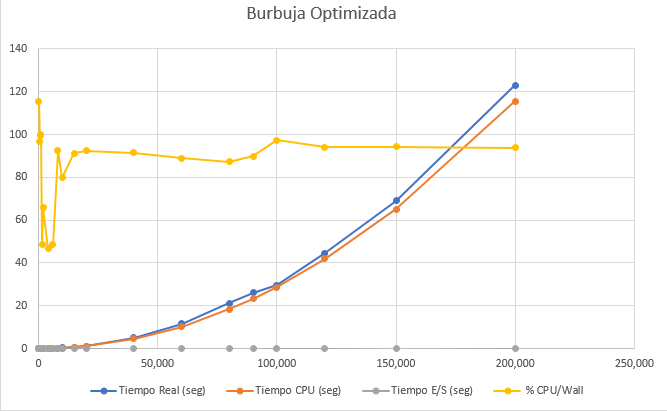
\includegraphics[scale=1.0]{images/Graficas/BO.PNG}
                \end{figure}
    		\newpage
    		\subsubsection{Aproximaciones Polinomiales}
        		    \begin{figure}[h!]
                    \centering
                   \subfigure{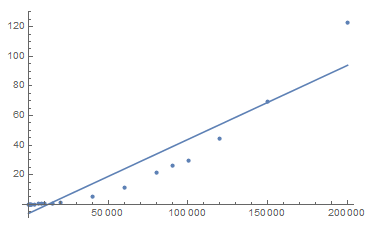
\includegraphics[width=0.61\textwidth]{Practica1/images/BSOpol1.PNG}
                   \caption*{\textbf{Grado 1: $-6.14724 + 0.000500917 x$}}}
    
    
                   \subfigure{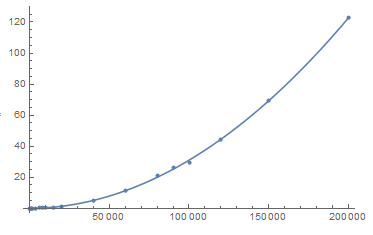
\includegraphics[width=0.61\textwidth]{Practica1/images/BSOpol2.PNG}
                   \caption*{\textbf{Grado 2: $-0.0288546 + 7.55172\times10^{-6} x + 3.03448\times10^{-9} x^2$}}}
                   \\
        		  \subfigure{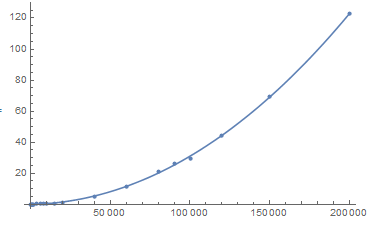
\includegraphics[width=0.61\textwidth]{Practica1/images/BSOpol3.PNG}
                   \caption*{\textbf{Grado 3: $-0.0998419 + 0.000020404 x + 2.84002\times10^{-9} x^2 + 6.79964\times10^{-16} x^3$}}}
                   \end{figure}
                    \newpage
                   \begin{figure}[h!]
                    \centering
        		   \subfigure{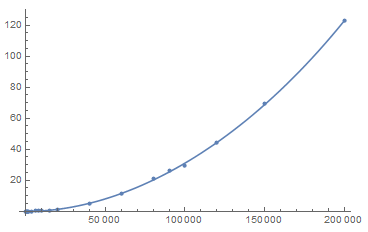
\includegraphics[width=0.61\textwidth]{Practica1/images/BSOpol4.PNG}
                   \caption*{\textbf{Grado 4: $-0.0214544 - 9.91421\times10^{-7} x + 3.44382\times10^{-9} x^2 - 
     4.55857\times10^{-15} x^3 + 1.37689\times10^{-20} x^4$}}}
                   
                   \subfigure{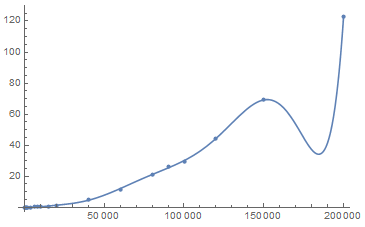
\includegraphics[width=0.61\textwidth]{Practica1/images/BSOpol8.PNG}
                   \caption*{\textbf{Grado 8:  $0.139882 - 0.000148344 x + 2.83418\times10^{-8} x^2 - 1.5772\times10^{-12} x^3 + 4.54088\times10^{-17} x^4 - 6.70478\times10^{-22} x^5 + 5.24334\times10^{-27} x^6 - 2.05962\times10^{-32} x^7 + 3.18722\times10^{-38} x^8$}}}
                \end{figure}
                \subsubsection{Evaluación de n's en Polinomios}
                            \begin{figure}[H]
        	            \centering
        	             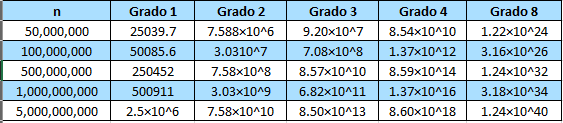
\includegraphics[scale=1]{images/NPols/nBSO.PNG}
                \end{figure}
            \newpage

		\subsection{Ordenamiento por inserción}
    		\subsubsection{Ejecución del algoritmo}
        		\begin{figure}[H]
        	            \centering
        	            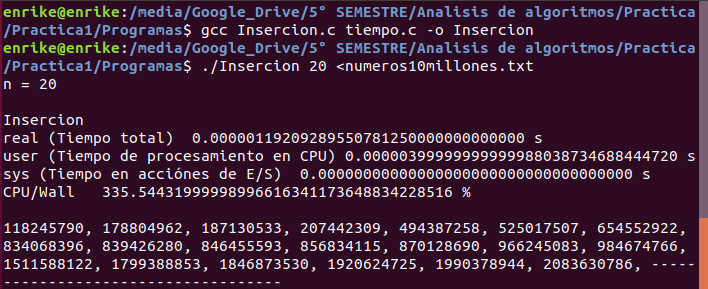
\includegraphics[scale=0.7]{images/Pruebas/insercion.png}
                \end{figure}
                
    		\subsubsection{Análisis Temporal}
    		    \begin{figure}[H]
        	            \centering
        	             \includegraphics[scale=1.0]{images/Tabla/Insercion.PNG}
                \end{figure}
    		\subsubsection{Gráfica de comportamiento}
    		    \begin{figure}[H]
        	            \centering
        	             \includegraphics[scale=1.0]{images/Graficas/Insercion.PNG}
                \end{figure}
    		\newpage
    		\subsubsection{Aproximaciones Polinomiales}
        		    \begin{figure}[h!]
                    \centering
                   \subfigure{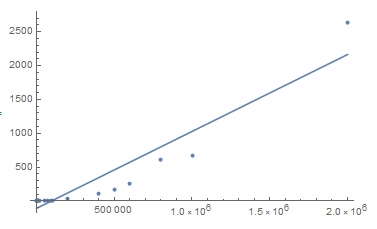
\includegraphics[width=0.61\textwidth]{Practica1/images/insercionpol1.PNG}
                   \caption*{\textbf{Grado 1: $-108.55 + 0.00113679 x$}}}
    
    
                   \subfigure{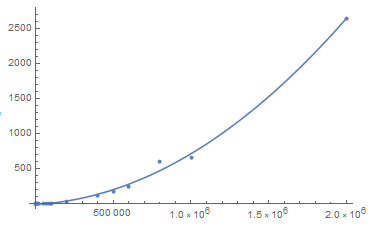
\includegraphics[width=0.61\textwidth]{Practica1/images/insercionpol2.PNG}
                   \caption*{\textbf{Grado 2: $-5.13494 + 0.0001174 x + 6.03912\times10^{-10} x^2$}}}
                   \\
        		  \subfigure{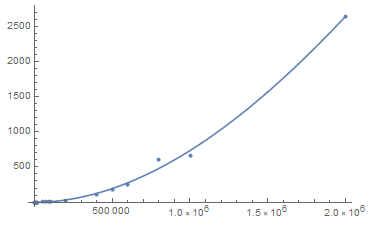
\includegraphics[width=0.61\textwidth]{Practica1/images/insercionpol3.PNG}
                   \caption*{\textbf{Grado 3: $-1.40767 + 0.0000152309 x + 7.89524\times10^{-10} x^2 - 6.82285\times10^{-17} x^3$}}}
                   \end{figure}
                    \newpage
                   \begin{figure}[h!]
                    \centering
        		   \subfigure{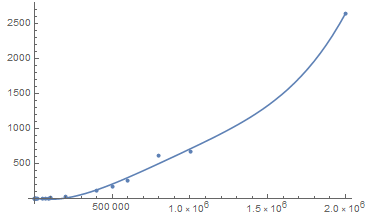
\includegraphics[width=0.61\textwidth]{Practica1/images/insercionpol4.PNG}
                   \caption*{\textbf{Grado 4: $7.34056 - 0.000400925 x + 2.35585\times10^{-9} x^2 - 1.76108\times10^{-15} x^3 + 5.06409\times10^{-22} x^4$}}}
                   
                   \subfigure{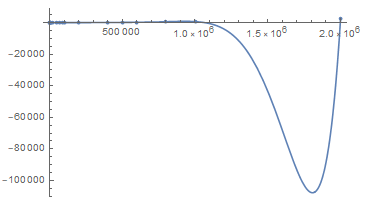
\includegraphics[width=0.61\textwidth]{Practica1/images/insercionpol8.PNG}
                   \caption*{\textbf{Grado 8:  $0.42113 - 0.000104528 x + 3.68568\times10^{-9} x^2 - 3.03438\times10^{-14} x^3 + 1.42669\times10^{-19} x^4 - 3.43268\times10^{-25} x^5 + 4.27728\times10^{-31} x^6 - 2.55327\times10^{-37} x^7 + 5.5625\times10^{-44} x^8$}}}
                \end{figure}
                \subsubsection{Evaluación de n's en Polinomios}
                            \begin{figure}[H]
        	            \centering
        	             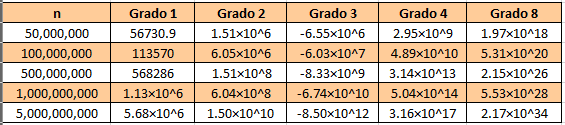
\includegraphics[scale=1]{images/NPols/nInsercion.PNG}
                \end{figure}
\newpage

		\subsection{Ordenamiento por selección}
    		\subsubsection{Ejecución del algoritmo}
        		\begin{figure}[H]
        	            \centering
        	            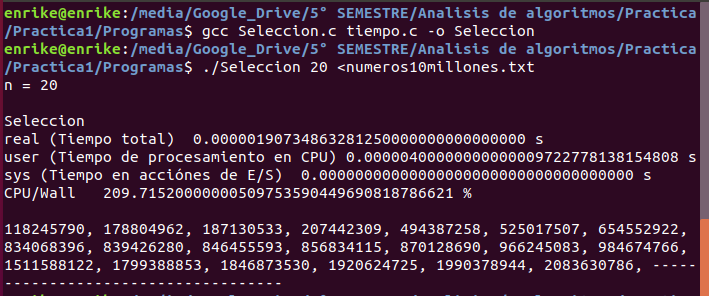
\includegraphics[scale=0.7]{images/Pruebas/seleccion.png}
                \end{figure}
    		\subsubsection{Análisis Temporal}
    		    \begin{figure}[H]
        	            \centering
        	             \includegraphics[scale=1.0]{images/Tabla/Seleccion.PNG}
                \end{figure}
    		\subsubsection{Gráfica de comportamiento}
    		    \begin{figure}[H]
        	            \centering
        	             \includegraphics[scale=1.0]{images/Graficas/Seleccion.PNG}
                \end{figure}
    		\newpage
    		\subsubsection{Aproximaciones Polinomiales}
        		    \begin{figure}[h!]
                    \centering
                   \subfigure{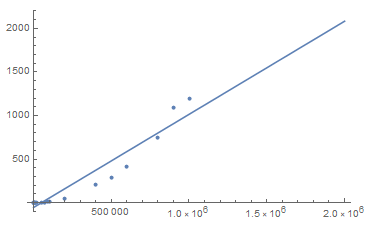
\includegraphics[width=0.61\textwidth]{Practica1/images/seleccionpol1.PNG}
                   \caption*{\textbf{Grado 1: $-53.8503 + 0.00106898 x$}}}
    
    
                   \subfigure{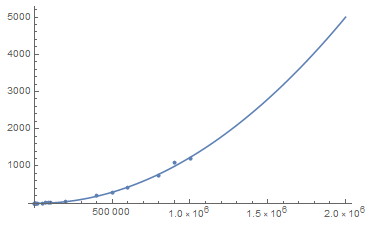
\includegraphics[width=0.61\textwidth]{Practica1/images/seleccionpol2.PNG}
                   \caption*{\textbf{Grado 2: $0.933709 - 0.0000347738 x + 1.26724\times10^{-9} x^2$}}}
                   \\
        		  \subfigure{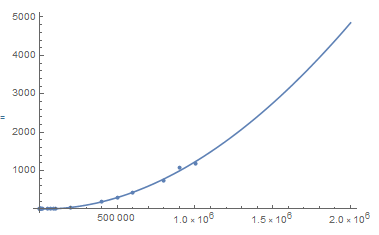
\includegraphics[width=0.61\textwidth]{Practica1/images/seleccionpol3.PNG}
                   \caption*{\textbf{Grado 3: $1.46243 - 0.0000567496 x + 1.33337\times10^{-9} x^2 - 4.6366\times10^{-17} x^3$}}}
                   \end{figure}
                    \newpage
                   \begin{figure}[h!]
                    \centering
        		   \subfigure{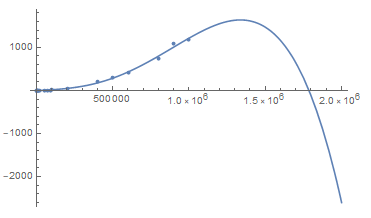
\includegraphics[width=0.61\textwidth]{Practica1/images/seleccionpol4.PNG}
                   \caption*{\textbf{Grado 4: $-3.14247 + 0.000234829 x - 3.72062\times10^{-10} x^2 + 2.91292\times10^{-15} x^3 - 1.55504\times10^{-21} x^4$}}}
                   
                   \subfigure{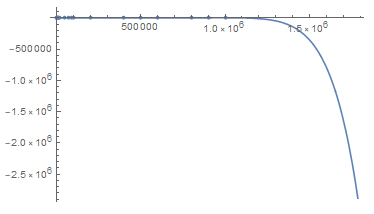
\includegraphics[width=0.61\textwidth]{Practica1/images/seleccionpol8.PNG}
                   \caption*{\textbf{Grado 8:  $-1.65689 + 0.00041812 x - 1.0197\times10^{-8} x^2 + 1.10428\times10^{-13} x^3 - 5.05429\times10^{-19} x^4 + 1.24266\times10^{-24} x^5 - 1.68957\times10^{-30} x^6 + 1.19325\times10^{-36} x^7 - 3.40375\times10^{-43} x^8$}}}
                \end{figure}
                \subsubsection{Evaluación de n's en Polinomios}
                            \begin{figure}[H]
        	            \centering
        	             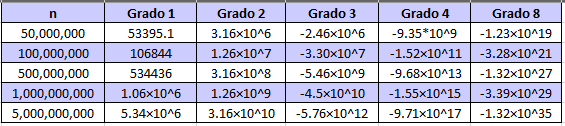
\includegraphics[scale=1]{images/NPols/nSelec.PNG}
                \end{figure}
\newpage

		\subsection{Ordenamiento Shell}
    		\subsubsection{Ejecución del algoritmo}
        		\begin{figure}[H]
        	            \centering
        	            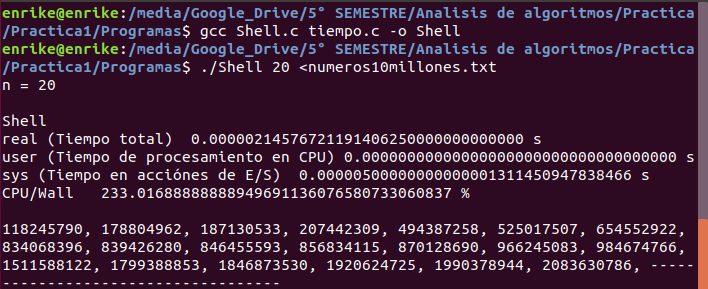
\includegraphics[scale=0.7]{images/Pruebas/shell.png}
                \end{figure}
    		\subsubsection{Análisis Temporal}
    		    \begin{figure}[H]
        	            \centering
        	             \includegraphics[scale=1.0]{images/Tabla/Shell.PNG}
                \end{figure}
    		\subsubsection{Gráfica de comportamiento}
    		    \begin{figure}[H]
        	            \centering
        	             \includegraphics[scale=1.0]{images/Graficas/Shell.PNG}
                \end{figure}
    		\newpage
    		
        		    \begin{figure}[h!]
        		    \subsubsection{Aproximaciones Polinomiales}
                    \centering
                   \subfigure{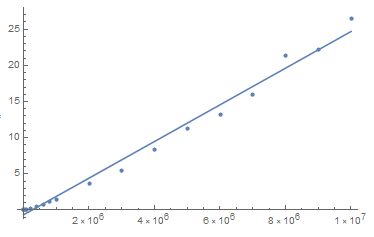
\includegraphics[width=0.6\textwidth]{Practica1/images/shellpol1.PNG}
                   \caption*{\textbf{Grado 1: $-0.642248 + 2.53478\times10^{-6} x$}}}
    
    
                   \subfigure{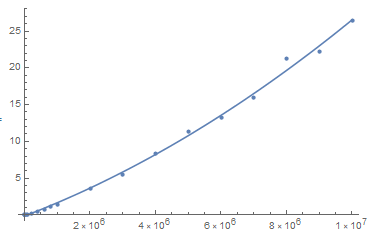
\includegraphics[width=0.6\textwidth]{Practica1/images/shellpol2.PNG}
                   \caption*{\textbf{Grado 2: $-0.128825 + 1.70604\times10^{-6} x + 9.60803\times10^{-14} x^2$}}}
    
        		  \subfigure{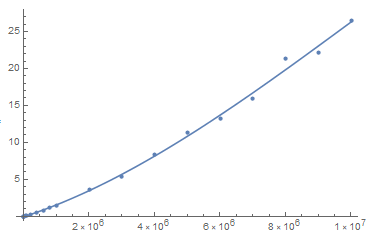
\includegraphics[width=0.6\textwidth]{Practica1/images/shellpol3.PNG}
                   \caption*{\textbf{Grado 3: $-0.0519355 + 1.42946\times10^{-6} x + 1.78285\times10^{-13} x^2 - 5.77542\times10^{-21} x^3$}}}
                   \end{figure}
                    \newpage
                   \begin{figure}[h!]
                    \centering
        		   \subfigure{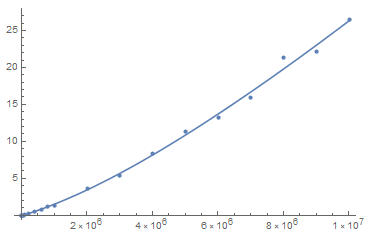
\includegraphics[width=0.61\textwidth]{Practica1/images/shellpol4.PNG}
                   \caption*{\textbf{Grado 4: $-0.0400139 + 1.35877\times10^{-6} x + 2.17949\times10^{-13} x^2 - 1.24843\times10^{-20} x^3 + 3.46719\times10^{-28} x^4$}}}
                   
                   \subfigure{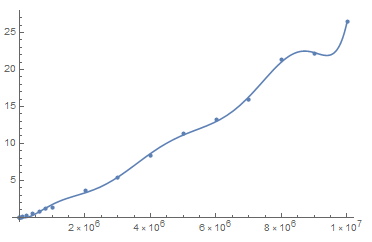
\includegraphics[width=0.61\textwidth]{Practica1/images/shellpol8.PNG}
                   \caption*{\textbf{Grado 8:  $0.0889081 - 2.02157\times10^{-6} x + 9.15851\times10^{-12} x^2 - 8.48395\times10^{-18} x^3 + 3.82072\times10^{-24} x^4 - 9.14639\times10^{-31} x^5 + 1.19178\times10^{-37} x^6 - 7.97176\times10^{-45} x^7 + 2.1411\times10^{-52} x^8$}}}
                \end{figure}
                \subsubsection{Evaluación de n's en Polinomios}
                            \begin{figure}[H]
        	            \centering
        	             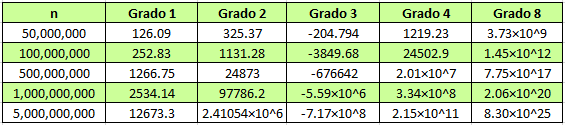
\includegraphics[scale=1]{images/NPols/nShell.PNG}
                \end{figure}
\newpage

		\subsection{Árbol binario de búsqueda}
		\subsubsection{Ejecución del algoritmo}
		    \begin{figure}[H]
    	            \centering
    	            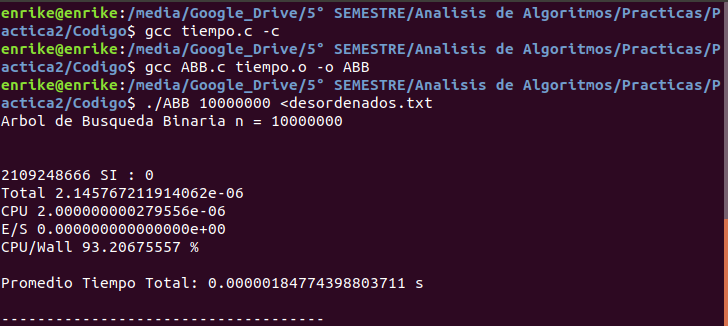
\includegraphics[scale=0.7]{images/Pruebas/abb.png}
            \end{figure}
		\subsubsection{Análisis Temporal}
		    \begin{figure}[H]
        	            \centering
        	             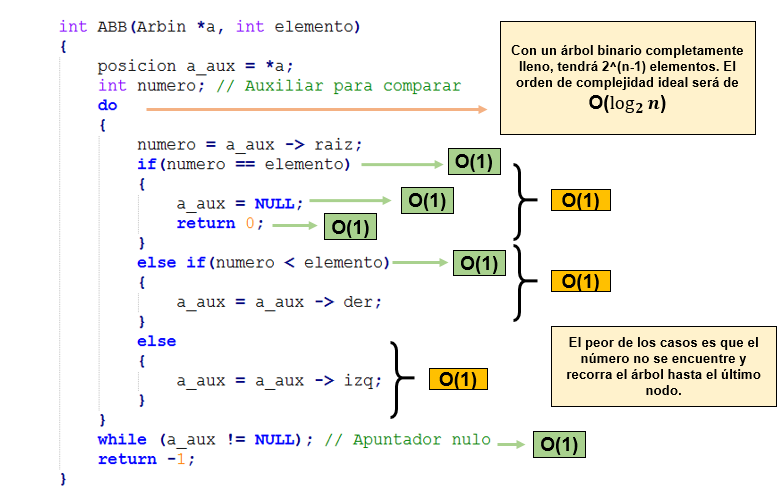
\includegraphics[scale=1.0]{images/Tabla/ABB.PNG}
                \end{figure}
		\subsubsection{Gráfica de comportamiento}
		    \begin{figure}[H]
        	            \centering
        	             \includegraphics[scale=1.0]{images/Graficas/ABB.PNG}
                \end{figure}
		\newpage
    		    \begin{figure}[h!]
    		    \subsubsection{Aproximaciones Polinomiales}
                \centering
               \subfigure{\includegraphics[width=0.61\textwidth]{Practica1/images/abbpol1.PNG}
               \caption*{\textbf{Grado 1: $-0.373011 + 1.53853\times10^{-6} x$}}}


               \subfigure{\includegraphics[width=0.61\textwidth]{Practica1/images/abbpol2.PNG}
               \caption*{\textbf{Grado 2: $-0.126987 + 1.14141\times10^{-6} x + 4.604\times10^{-14} x^2$}}}

    		  \subfigure{\includegraphics[width=0.61\textwidth]{Practica1/images/abbpol3.PNG}
               \caption*{\textbf{Grado 3: $-0.0615581 + 9.06049\times10^{-7} x + 1.15993\times10^{-13} x^2 - 4.91464\times10^{-21} x^3$}}}
               \end{figure}
               \clearpage
               \begin{figure}[h!]
                \centering
    		   \subfigure{\includegraphics[width=0.61\textwidth]{Practica1/images/abbpol4.PNG}
               \caption*{\textbf{Grado 4: $-0.0222793 + 6.73151\times10^{-7} x + 2.46674\times10^{-13} x^2 - 2.70187\times10^{-20} x^3 + 1.14236\times10^{-27} x^4$}}}
               
               \subfigure{\includegraphics[width=0.61\textwidth]{Practica1/images/abbpol8.PNG}
               \caption*{\textbf{Grado 8:  $0.000327011 + 2.62645\times10^{-7} x + 1.06888\times10^{-12} x^2 - 6.3221\times10^{-19} x^3 + 2.20885\times10^{-25} x^4 - 4.36496\times10^{-32} x^5 + 4.82736\times10^{-39} x^6 - 2.78724\times10^{-46} x^7 + 6.54442\times10^{-54} x^8$}}}
            \end{figure}
            \subsubsection{Evaluación de n's en Polinomios}
                        \begin{figure}[H]
        	            \centering
        	             \includegraphics[scale=1]{images/NPols/nABB.PNG}
                \end{figure}
            
\clearpage
        
		\subsection{Comparativa de tiempos reales y de CPU}
		\begin{itemize}
		    \item Con n = 200,000
		    \begin{figure}[h!]
                \centering
               \includegraphics[width=\textwidth]{Practica1/images/barras1.PNG}
            \end{figure}
		    \item Con n = 1,000,000
		    \begin{figure}[h!]
                
               \includegraphics[width=0.7\textwidth]{Practica1/images/barras2.PNG}
            \end{figure}
		    \item Con n = 10,000,000
		    \begin{figure}[h!]
                
               \includegraphics[width=0.5\textwidth]{Practica1/images/barras3.PNG}
            \end{figure}
		\end{itemize}
		
		
		\subsection{Comparativa de gráficas de comportamiento (Tiempo Real)}
		  \begin{figure}[H]
    	            \centering
    	            \includegraphics[scale=1]{images/Graficas/Comparacion.PNG}
            \end{figure}
		\newpage

		\begin{figure}[h!]
		\subsection{Comparativa de aproximaciones polinomiales}
                \centering
               \subfigure{\includegraphics[width=0.9\textwidth]{Practica1/images/comp1.PNG}
               \caption*{\textbf{Grado 1}}}
          \subfigure{\includegraphics[width=0.9\textwidth]{Practica1/images/comp2.PNG}
          \caption*{\textbf{Grado 2}}}
    		  \subfigure{\includegraphics[width=0.9\textwidth]{Practica1/images/comp3.PNG}
    		  \caption*{\textbf{Grado 3}}}
    		  \end{figure}
               \clearpage
               \begin{figure}[h!]
                \centering
    		   \subfigure{\includegraphics[width=0.9\textwidth]{Practica1/images/comp4.PNG}
    		   \caption*{\textbf{Grado 4}}}
               \subfigure{\includegraphics[width=0.9\textwidth]{Practica1/images/comp8.PNG}
               \caption*{\textbf{Grado 8}}}
            \end{figure}
        

		\section{Cuestionario}
		    \begin{enumerate}
		        \item ¿Cuál de los 5 algoritmos es más fácil de implementar?\\
		        Para nosotros, el más fácil de implementar fue el de inserción, debido a que fue sencillo comprender su funcionamiento. Los algoritmos de burbuja también tienen un nivel de implementación claro.\\
		        \item ¿Cuál de los 5 algoritmos es el más difícil de implementar?\\
		        Debido a que se requiere un análisis de apuntadores, consideramos que el árbol de búsqueda binaria podría ser el más complicado de implementar.\\
		        \newpage
		        \item ¿Cuál algoritmo tiene menos complejidad temporal?\\
		        Una vez realizadas las pruebas, el algoritmo con menor complejidad temporal fue el de árbol de búsqueda binaria, seguido por el de Shell.\\
		        
		        \item ¿Cuál algoritmo tiene mayor complejidad temporal?\\
		        En la teoría, con números muy grandes debería ser indiferente la complejidad temporal, sin embargo, los algoritmos de ordenamiento de burbuja demostraron ser los menos eficientes, ya que tan solo llegar a ordenar 200,000 números tomaba más tiempo en comparación con la misma cantidad de números con los otros algoritmos de ordenamiento.\\
		        
		        \item ¿Cuál algoritmo tiene menor complejidad espacial? ¿Por qué?\\
                Existen dos que cumplen esta característica: el de burbuja simple y el de inserción, pues ambos hacen uso de únicamente un arreglo y 3 variables de control de las posiciones del arreglo, por lo que de entre todos estos consumen menor memoria.\\
		        
		        \item ¿Cuál algoritmo tiene mayor complejidad espacial? ¿Por qué?\\
		        En este caso observamos que el algoritmo de árbol de búsqueda binaria tuvo una mayor complejidad espacial, debido a que hace uso de estructuras del lenguaje C, apuntadores de memoria, y reasigna memoria dinámica a una variable de tipo Arbin cada vez que se realiza una inserción, siendo esta un nodo de aproximadamente tamaño n/2 en cada ramificación. \\
		        
		        
		        \item ¿El comportamiento experimental de los algoritmos era el esperado? ¿Por qué?\\
		        Si, esperábamos que los algoritmos de burbuja fuesen los que demostrasen los resultados menos favorables, así como que los algoritmos Shell y árbol binario tuviesen los mejores resultados. Esto debido al análisis previo a la práctica.\\
		        
		        \item ¿Sus resultados experimentales difieren mucho de los del resto de los equipos? ¿A que se debe?\\
		        No, a pesar de las diferentes capacidades de cada computadora, los resultados generales fueron similares; los algoritmos de burbuja fueron los menos favorables y el árbol binario fue el más eficiente.\\
		        
		        \item ¿Existió un entorno controlado para realizar las pruebas experimentales? ¿Cuál fue?\\
		        Si, se realizaron los ordenamientos con distintos tamaños de problema (n's) según el algoritmo, todos al mismo tiempo. Todos los algoritmos fueron probados en la misma máquina al momento de realizar las gráficas comparativas.\\
		        
		        \item ¿Qué recomendaciones darían a nuevos equipos para realizar esta práctica?\\
		        Realizar una investigación previa a la práctica acerca del funcionamiento e implementación de cada algoritmo, de esta manera, cada integrante conoce el funcionamiento de cada algoritmo sin la necesidad de realizar la implementación. Realizar comentarios en el código puede ser importante, pero es más sencillo si el nombre de las variables explica el código mismo.
		        
		    \end{enumerate}
	% /////////////////////////////////////////////////////////
	%							ANEXO
	% ////////////////////////////////////////////////////////
	\newpage
	\section{Anexos}
	
	\textbf{NOTA: Para ejecutar todas las pruebas de todos los algoritmos ejecutar el archivo script.sh con el siguiente comando e una terminal dentro de la carpeta de los códigos fuente: sh script.sh}

		\subsection{Burbuja simple}
		    \inputminted{c++}{Code/BurbujaSimple.c}

		\subsection{Burbuja Optimizada}
		    \inputminted{c++}{Code/BurbujaOptimizada.c}
		    \newpage
		\subsection{Ordenamiento por inserción}
			\inputminted{c++}{Code/Insercion.c}
		    
		\subsection{Ordenamiento por selección}
			\inputminted{c++}{Code/Seleccion.c}
		    
		\subsection{Ordenamiento Shell}
			\inputminted{c++}{Code/Shell.c}
		    
		\subsection{Árbol binario de búsqueda}
		\begin{itemize}
		    \item[\checkmark] Archivo .C 
		        \inputminted{c++}{Code/ABB.c}
		    \item[\checkmark] Archivo .H
		        \inputminted{c++}{Code/Arbin.h}
		\end{itemize}
		    
		\subsection{Script de Compilación}
		 \inputminted{c++}{Code/script.c}
			
	% /////////////////////////////////////////////////////////
	%						BIBLIOGRAFIA
	% ////////////////////////////////////////////////////////
	
	\section{Bibliografía}
	
	$[1]$ E. A. Franco Martínez, “Practica 01 : Pruebas a posteriori (Algoritmos de Ordenamiento)” Análisis de Algoritmos, Escuela Superior de Computación, Instituto Politécnico Nacional,
    Ciudad de México, México, Practica01.pdf, Sep. 2018
  
    $[2]$ (2018) WolframAlpha. Accessed september 2018. [Online]. \\Available: http://www.wolframalpha.com/

	\nocite{ref2}
	\bibliography{referencias}
     
\end{document}